\section{Modelo usando Propiedades Estructurales de la Proteína}

En el primer trabajo de predicción realizado con este dataset  se intentó aumentar la cantidad de ejemplos, o ``filas'', para mejorar la precisión pero no hubieron mayores avances en este sentido \textbf{[Citar Moreno et al.]}. Por lo tanto en este trabajo nos proponemos sumar ``columnas'', es decir, nuevas variables que describan mejor las variantes.

Una de las primeras cuestiones que quisimos abordar fue encontrar nuevas fuentes de información de carácter estructural de las proteínas que enriquecieran el dataset de VarQ. 



Por esta razón, una vez obtenidas nuevas variables usando ProtParam, como también las características relativas a los aminoácidos encontradas en SNVBox, generamos un modelo usando estos atributos con el dataset Humsavar. En el caso de los atributos relativos a los aminoácidos, estas variables contienen información sobre los cambios entre un aminoácido y su variante, por ejemplo el cambio en la hidrofobicidad, la polaridad o la carga. También contienen diferentes matrices de sustitución, como BLOSUM o PAM. Estas matrices son utilizadas para alineamientos múltiples de secuencias (MSA, por sus siglas en inglés) y asignan diferentes ``pesos'' a los pares de sustitución teniendo en cuenta la probabilidad de que ocurra. Por otro lado, las características encontradas en ProtParam permiten calcular también los cambios que se generan no sólo en la posición del cambio de aminoácido sino de su contexto en la subsecuencia resultante. 

% \todo{TODO: Acá va una descripción de las variables}

% \subsection{Correlación}

\begin{figure}[H]
    \centering
    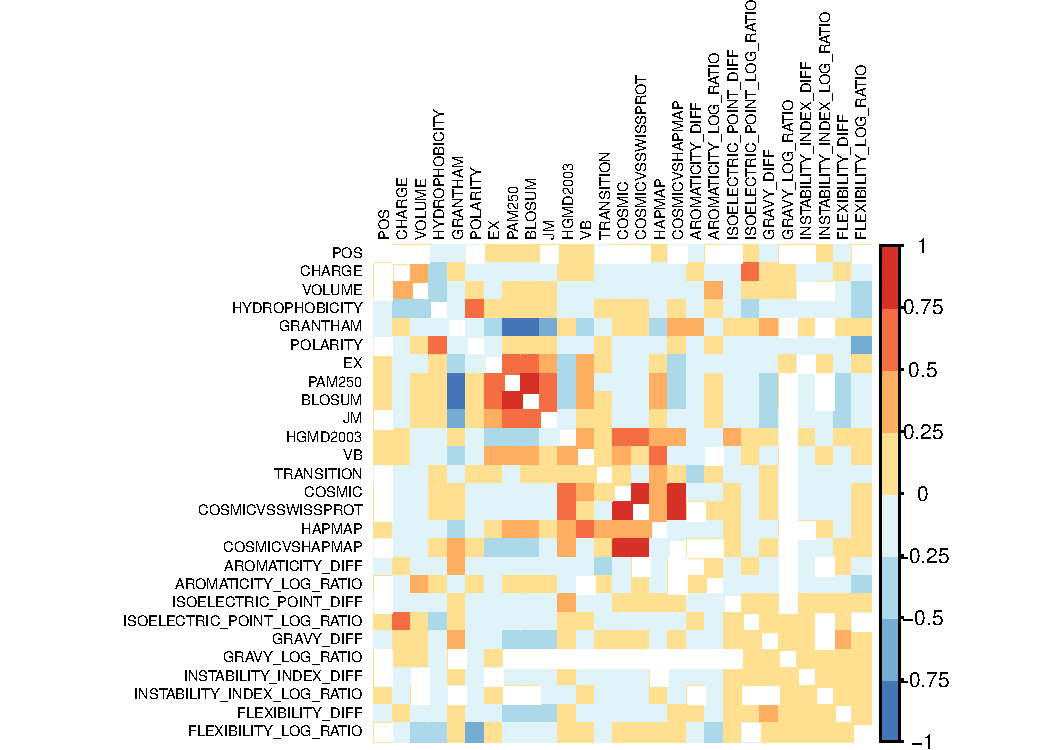
\includegraphics[scale=0.8]{documents/latex/figures/3/corrplot_1.pdf}
    \caption{Test de Correlación de Pearson (Significación: 0,05). Los valores en blanco poseen un p-valor por debajo del nivel de significación. Se puede observar que GRANTHAM se encuentra altamente anti-correlacionado con las matrices PAM y BLOSUM, mientras que estas se encuentran correlacionadas al igual que con EX.}
    \label{fig:corrplot_1}
\end{figure}

Este dataset está compuesto por 68508 ejemplos y 28 variables incluyendo la variable de respuesta, de los cuales 39653 son polimorfismos, o variantes ``inocuas'' (no se encontró reportes de enfermedades relacionadas a este cambio en la literatura), y 28855 variantes asociadas a alguna enfermedad. Este dataset se dividió en 20 pares de conjuntos de entrenamiento y evaluación, como se explica en la sección 2.3, con el objetivo de obtener la varianza de nuestros resultados. 
Para entrenar el modelo usamos un predictor \textit{Random Forest} con búsqueda de hiperparámetros ``en cuadrícula'' (\textit{Grid-Search}). 

A partir de este modelo se obtuvo un AUC de 0,71, que supera lo obtenido por el modelo usando el dataset VarQ. Las otras métricas permiten dar cuenta de una baja precisión con respecto a las variantes patógenas (lo cual es de esperar, dado que son nuestro mayor problema a identificar) pero una buena sensibilidad, lo que indica una gran cantidad de falsos positivos pero no tantos falsos negativos.

\begin{table}[H]
\centering
\begin{tabular}{llll}
              & Precisión & Sensibilidad & F1-score \\
Patógenas     & 0.34      & 0.63   & 0.44     \\
Polimorfismos & 0.88      & 0.67   & 0.76     \\
Media         & 0.76      & 0.67   & 0.70     \\
              &           &        &         
\end{tabular}
\caption{Resultado de las distintas métricas.}
\label{my-label}
\end{table}

% \subsection{Resultados}

\begin{figure}[H]
    \centering
    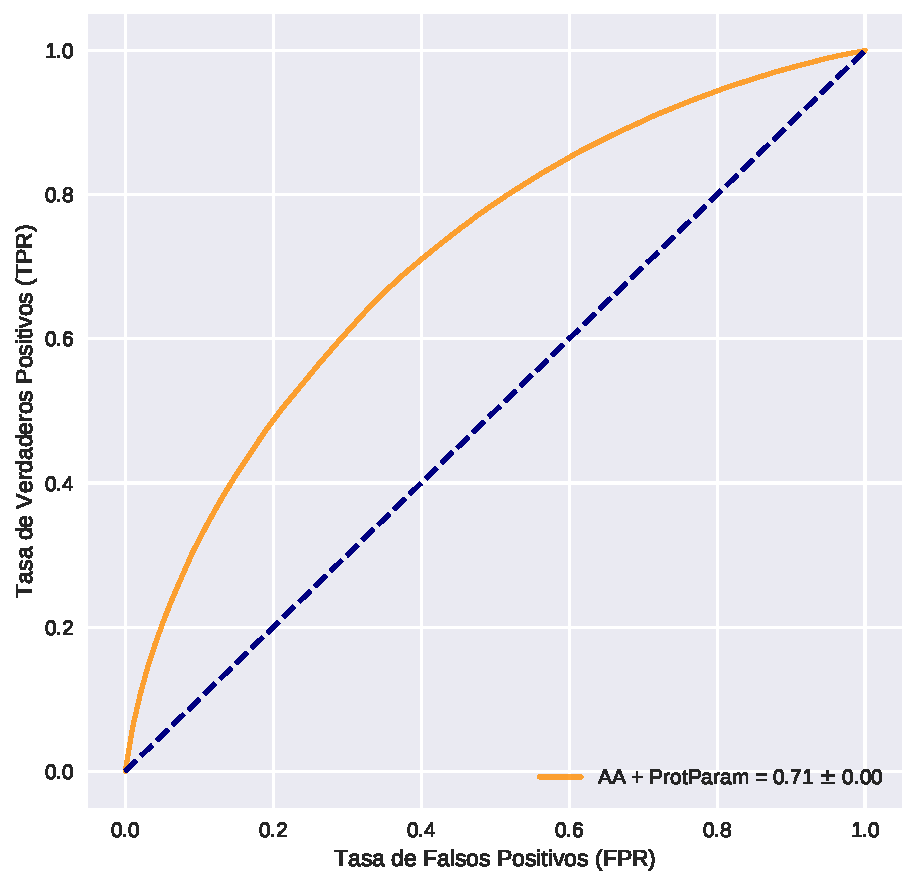
\includegraphics[scale=0.73]{documents/latex/figures/3/auc_1.pdf}
    \caption{Curva AUC del algoritmo Random Forest. La línea punteada corresponde a un predictor \textit{Random}.}
    \label{fig:auc_1}
\end{figure}


% \subsection{Importancia de los atributos}


El algoritmo nos permite identificar los mejores atributos dado su rango en cada uno de los árboles del clasificador. En este caso, podemos ver que los primeros cuatro atributos refieren a matrices de sustitución. El quinto atributo más importante, HGMD2003, significa el número de veces que la mutación ocurrió en la base de datos de mutaciones genéticas humanas, por lo que podemos decir, como en los 4 primeros atributos, que aporta información sobre la ``rareza'' de una mutación. Recién en el sexto puesto aparece una característica sobre el aminoácido reemplazado (cambio en la polaridad), seguido por otra matriz de sustitución (JM), y los últimos 3 también se refieren a cambios aportados por el nuevo aminoácido.

\begin{figure}[H]
    \centering
    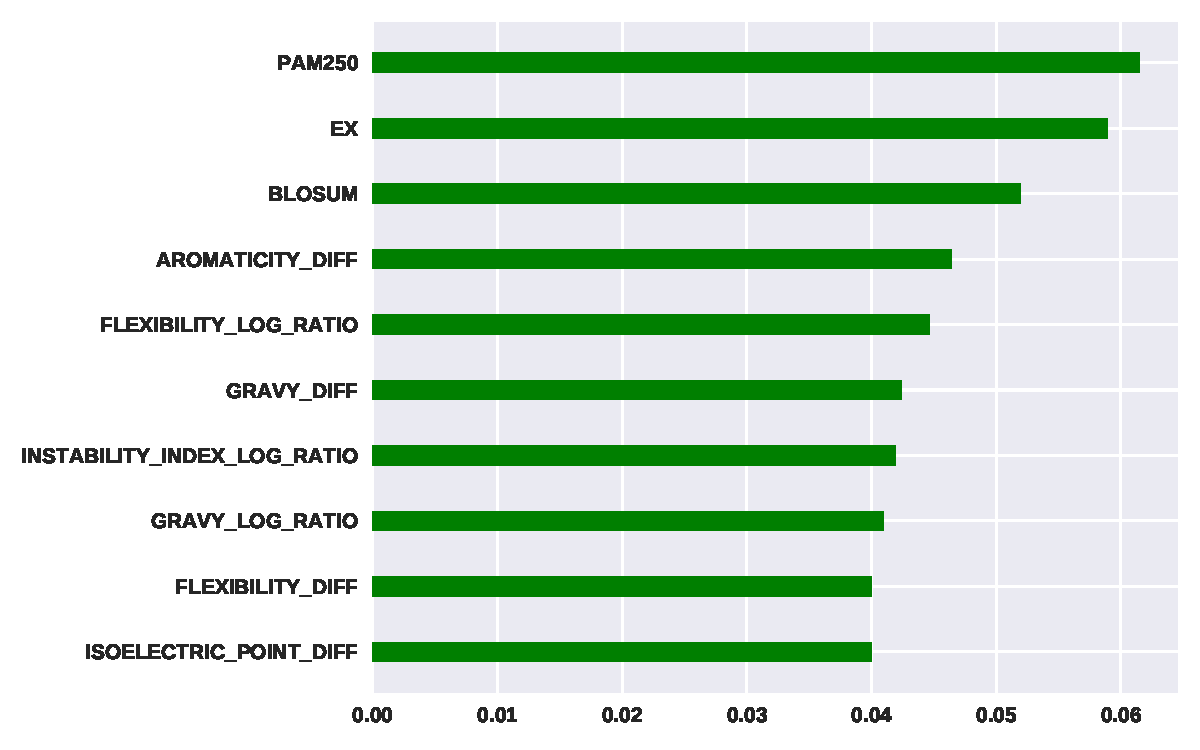
\includegraphics[scale=0.73]{documents/latex/figures/3/importance_1.pdf}
    \caption{Los 10 atributos más importantes.}
    \label{fig:importance_1}
\end{figure}


\subsection{Uniendo las variables al Dataset VarQ}

\section{Modelo usando Variables Genómicas}
% \subsection{Descripción}
% \subsection{Correlación}

% \subsection{Resultados}

\section{Uniendo los dos Mundos}

